\ctable[caption={Studying a problem at multiple scales},
		label={fig:scales},
		width=5.5cm,
		figure]{c}{\tnote[]{Generic idea of renormalization. First the problem is solved at the
		largest scale. This block is divided into four sub blocks, where the process is repeated
		until unity is reached.}}{\FL
			\includegraphics[width=5cm]{fig/ising.png}
		\LL}
<<<<<<< renorm_method.tex
At the heart of the method proposed in this work to solve the TSP is the
renormalization theory \cite{yoshiyuki1995nms}. This theory originates from theoretical physics where
it is used to study the observerd mutations of physical system. These changes
are observed by considering the problem at different scales. This concept is
illustrated in Fig. \ref{fig:scales}. In this figure the problem is initially
divided into four parts. These parts on their own can again be divided into
four parts. This process of dividing cells can be repeated until the scale is
small enough to study the original problem.

This idea is mapped onto the TSP problem. The total square in figure
\ref{fig:scales} can be seen as the total area where the cities are located.
To estimate the shortest route, the problem is first approached at a large
scale. To find the shortest route the pane is magnified until the route is
found. The procedure is illustrated in Fig. \ref{fig:renormalization}. The
image in the picture in the upper left corner is the basic block. This basic
block consists of four cells, and can be viewed as the four parts in which the
problem is divided to a smaller scale. A cell spans a part of the
pane, and can be enabled or not. If a cell contains one or more cities it is
enabled and thereby specifies to the system that the TSP has to visit the area
spanned by the cell.

The general idea of the algorithm is to solve the TSP problem
for the initial block. This can easily be achieved by iterating over all the
possibilities at almost no computing cost. Once done, the problem can be
analyzed at a smaller scale by dividing the blocks into four sub blocks.
Together with some information acquired from the larger block, the TSP 
problem can again be solved for the four sub blocks. This process is
repeated until there is at most one city in a cell, and the estimated optimal
tour is known. 

The following subsection describes the algorithm in more detail.

\subsection{Preprocessing step}
\ctable[caption={An illustration of how the renormalization algorithm works},
	label={fig:renormalization},
	figure]{c}{\tnote[]{
	\begin{enumerate}
	\item[(A)] Determine the optimal route in a basic block. The dashed
	lines are the edges which can be traversed. The open circles are border
	points and the closed circles are cell points.
	\item[(B)] Based on the starting and end border node in a block, lookup the
	optimal path visiting the cells where at least one city is located.\\
	\item[(C)] Divide the block into four sub blocks(Each cell is converted into a basic block)
	, use the crossings of the route
	with the borders of a cell (The X) as new starting and end nodes.\\
	\item[(D)] These sub blocks are treated as a block again, and the process is repeated from
	picture B. This dividing continues until at most one city is located in each cell.
	\end{enumerate}}}{\FL
	\includegraphics[width=7cm]{fig/renormalization.pdf}
	\LL}

The preprocessing step reduces the computations necessary to find the optimal
route for each block. In this step the optimal path for each possible
configuration is stored in a lookup table for later use. During the execution
of the rest of the algorithm these values can be used together with the
information if cells are enabled and the border points where the route begins
and ends.

To find the shortest route through a block it is modelled as a graph. The
nodes represent the border points and the points in the centre of each cell.
The nodes are interconnected with multiple edges. Each node which represents a
border point is connect to the node which represents the closest cell centre.
Moreover, nodes which represent cell centres are connected to the other edges.
An example of this setup is displayed in Fig. \ref{fig:renormalization}. The
shortest route can then be find using a breadth first search. For this search,
the length is computed of each possible path without cycles in the graph 
which connects the entry point to the exit point. The shortest route among the
computed set of points is than elected.

\subsection{First iteration}
The first iteration starts with one block consisting of four cells. In such a
block a subset of at least 3 cells needs to be occupied to form a starting
tour. The cells where at least one city is located, are connected to form a
shortest tour. This tour is an easy connection of the cities, and all the
possible routes between them do not need to be investigated.

\subsection{Further iterations}
<<<<<<< renorm_method.tex
\ctable[caption={The first four iterations on d198.tsp},
		label={fig:iterations},
		width=7.5cm,
		figure]{cc}{\tnote[]{The renormalization starts with a basic form, a 
		square or a triangle. This slowly refines to the real tour through the 
		cities}}{\FL
			\includegraphics[width=3.5cm]{fig/it2.pdf} &
			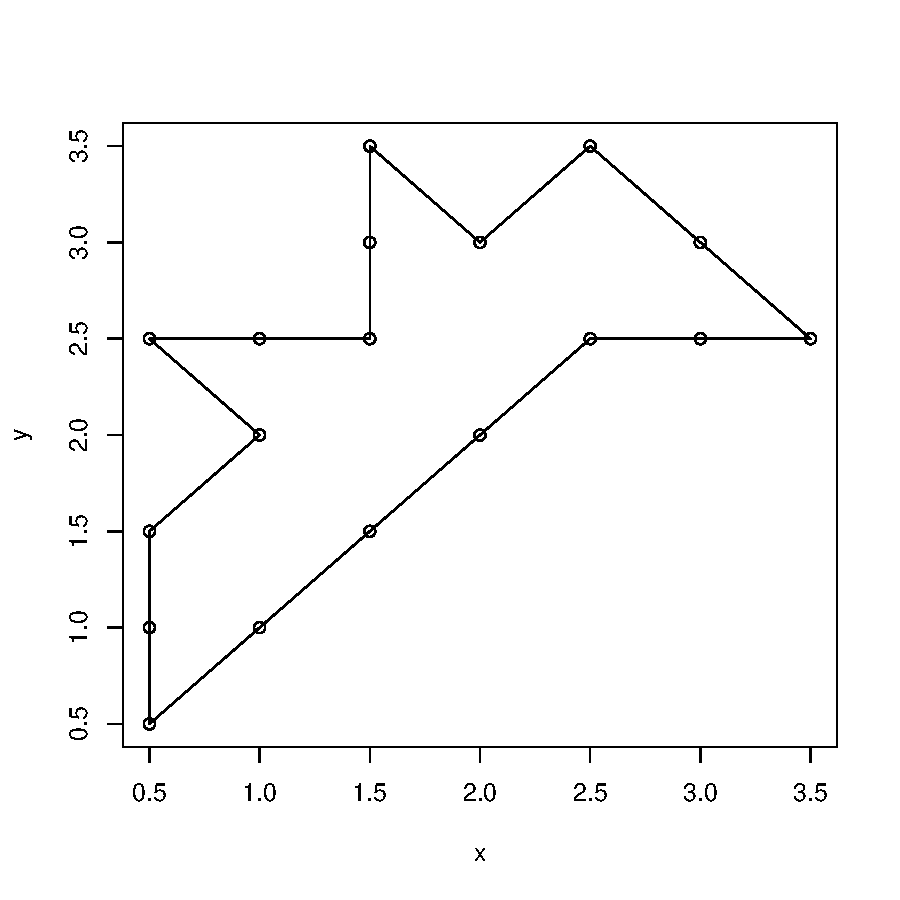
\includegraphics[width=3.5cm]{fig/it4.pdf} \NN
			\includegraphics[width=3.5cm]{fig/it8.pdf} &
			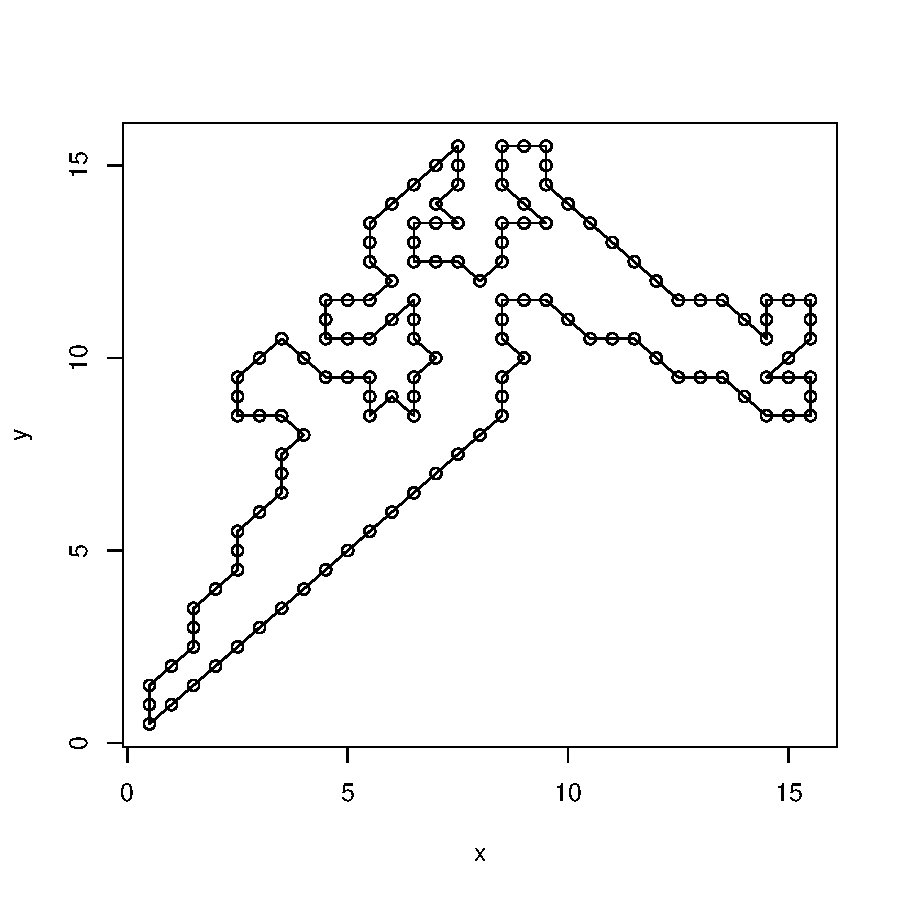
\includegraphics[width=3.5cm]{fig/it16.pdf} 
			\LL}


When the first iteration is finished the earlier used blocks can be used to
compute a new approximation of the shortest route at a smaller scale. The
smaller scale is obtained by converting each cell to a block and dividing
these blocks into four cells. Instead of iterating over all the sub blocks,
which can be quite time consuming at a very small scale, only the blocks which
contain at least one city in the previous estimated shortest tour are
used in the calculation. This reduces the necessary memory in the order of the
size of the problem.

The information which is retrieved from the previous scale are the crossing
points of the previous optimal path through the block. This optimal path can
be seen in figure \ref{fig:renormalization}B.  These crossing points are at
the places, where the edges of the path, pass the borders of one of the cells.
This is illustrated in figure \ref{fig:renormalization}C. These crossing
points, calculated in advance during the preprocessing stage, are used as start and
ending point in the sub block. The optimal path between the starting and
endpoint is retrieved, and placed in the sub block. The sub block is now a block
on its own again, and can be used in the next scale.

\subsection{Retrieving the estimate of the shortest tour}
This process, which looks like zooming in on a microscope, is repeated until
 unity is reached. Unity is defined as the case where each cell contains at most one
city. In this case the estimated shortest path can be retrieved directly by following 
the tour through the basic blocks.
In figure \ref{fig:iterations} the first four iterations of the algorithm on
$d198.tsp$ is shown. What is clear from this picture is that the route is
refined in each iteration, until it exactly maps on the estimation  of the
shortest optimal tour.

\ctable[caption={The first four iterations on d198.tsp},
		label={fig:iterations},
		width=7.5cm,
		figure]{cc}{\tnote[]{The renormalization starts with a basic form, a 
		square or a triangle. This slowly refines to the real tour through the 
		cities}}{\FL
			\includegraphics[width=3.5cm]{fig/it2.pdf} &
			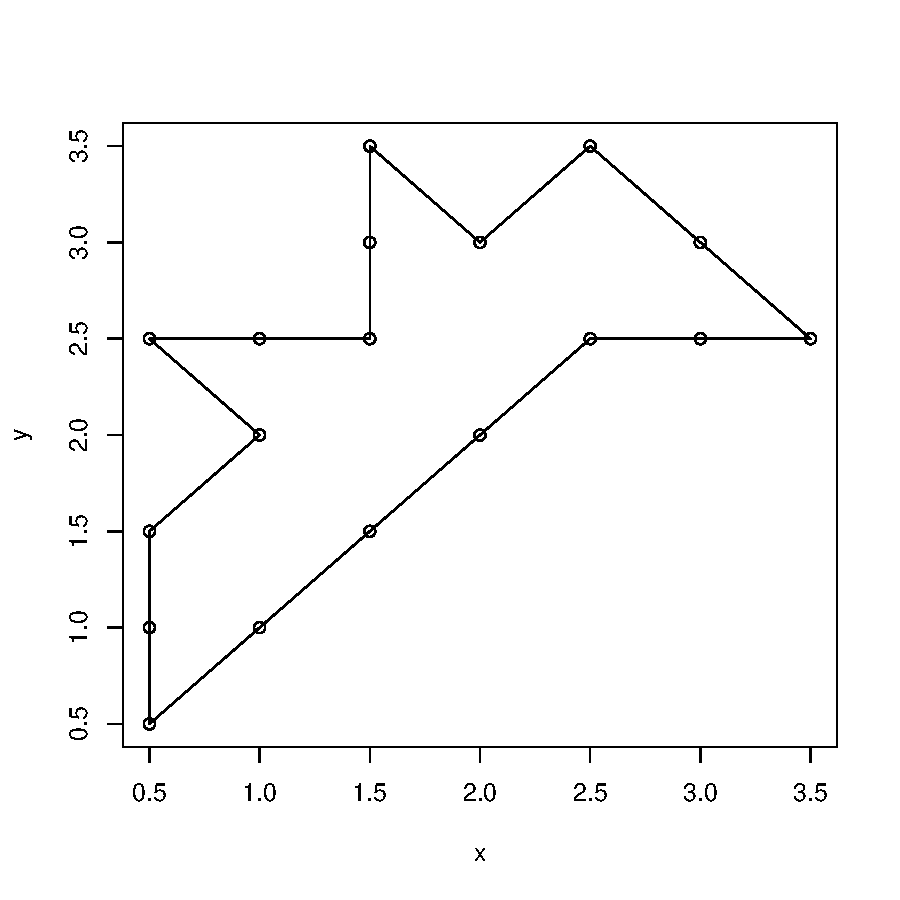
\includegraphics[width=3.5cm]{fig/it4.pdf} \NN
			\includegraphics[width=3.5cm]{fig/it8.pdf} &
			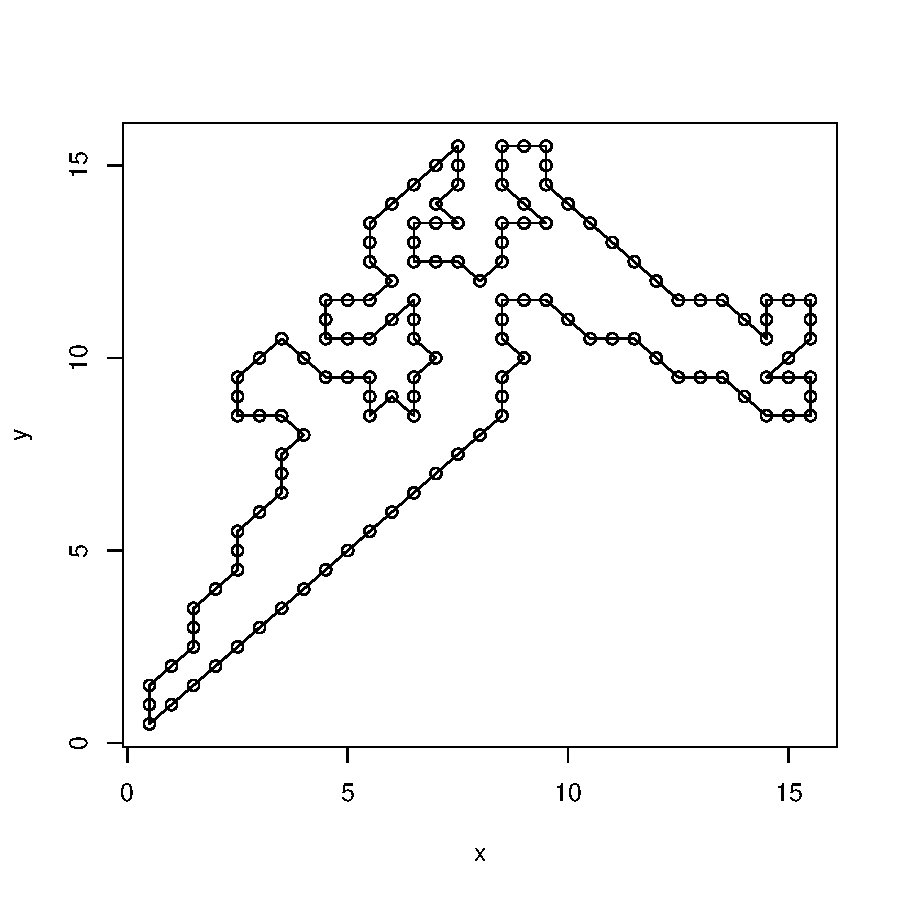
\includegraphics[width=3.5cm]{fig/it16.pdf} 
			\LL}

\subsection{Parallelization}
This algorithm can be extended for parallel execution. The foundation for
parallelism is in the observation that if the problem is decreased into a smaller scale, 
all the blocks are divided into four sub blocks independently. So if the code needs
to be parallelized the following approach can be taken:

\begin{enumerate}
\item First perform some iterations on a single process. This is done until
there are sufficient number of blocks for all the processes
\item Distribute the blocks over the processes, each process should have one
connected part of the tour.
\item Each process can now recursively divide these blocks into sub blocks,
until unity is reached.
\item The cities which are visited in the part of a single process are
retrieved and send back to the initiating process. The initiating process can collect the
data and output the total tour.
\end{enumerate}

This approach has a high potential of parallelism, since no communication is
needed. There is a pitfall however. If the blocks are shared equally it does
not have to mean that the work is equally divided. In a worst case scenario a
small group of processes can have a large set of all the cities. This problem
can be reduced if there is a process which performs load balancing by shifting
blocks, or sending one small set of blocks to a process at the time.

% vim:ft=tex:spell spelllang=en:autoindent
